\documentclass[16 pt]{amsart}
\usepackage{amscd,amsmath,amsthm,amssymb}
\usepackage{enumerate,varioref}
\usepackage{epsfig}
\usepackage{graphicx}
\usepackage{mathtools}
\usepackage{tikz}
\newtheorem{thm}{Theorem}
\newtheorem{cor}[thm]{Corollary}
\newtheorem{lem}[thm]{Lemma}
\newtheorem{prop}[thm]{Proposition}
\theoremstyle{definition}
\newtheorem{defn}[thm]{Definition}
\theoremstyle{remark}
\newtheorem{ex}[thm]{Example}
\newtheorem{rem}[thm]{Remark}
\numberwithin{equation}{subsection}
\newcommand{\R}{\mathbb{R}}
\newcommand{\Z}{\mathbb{Z}}
\newcommand{\C}{\mathbb{C}}
\newcommand{\Q}{\mathbb{Q}}
\newcommand{\lh}{\lim_{h\rightarrow 0}}
\begin{document}

\title{Midterm 2 Maths 140 Autumn 2016 \\ DePaul University\\Dr. Alexander}
\maketitle
You have 90 minutes to complete this exam.  Calculators are allowed, but no other electronic devices are permitted.  Please write all your answers in complete, legible sentences, and show all your work to receive full credit.  There are seven (7) problems here.  You may choose to do any six (6) of them.  
\vspace{1in}


%table
\begin{center}
  \begin{tabular}{ c | c }
    Problem & Score\\
    \hline
    &\\
    1&\\
    &\\
    2&\\
    &\\
    3&\\
    &\\
    4&\\
    &\\
    5&\\
    &\\
    6&\\
    &\\
    7&\\
    &\\
    Bonus&\\
    &\\
    \hline 
    &\\    
    Total& 
 \end{tabular}
\end{center}

\newpage 
Problem 1. Let $A$ and $B$ be two sets and the universal set be $\mathcal{U}$.  Prove the following statement:
\[
A^c \cup B^c = (A\cap B)^c
\]

\vspace{1in}

Solution 1: Let's do this in the old fashioned set theoretic way.  First of all, let's suppose that $x\in A^c \cup B^c$ this means that $x$ is in at least one of $A^c$ or $B^c$.  In particular, if $x\in A^c$ then $x\notin A$.  Since $x$ is not an element of $A$ this means it will not be an element of $A\cap B$.  So if $x\in A^c$ then it is in $(A\cap B)^c$.  Similarly for $x\in B^c$ this means $x\in (A\cap B)^c$.  So we have just shown

\[
A^c \cup B^c \subseteq (A\cap B)^c
\]

Now let's show the other subset inclusion.  Suppose $x\in(A\cap B)^c$ this means $x$ fails to be in at least one of $A$ or $B$.
If $x\notin A$ then $x\in A^c$ and thus $x\in A^c\cup B^c$.  On the other hand, if $x\notin B$ then $x\in B^c$ and thus $x\in A^c\cup B^c$.  In either case we've shown
\[
(A\cap B)^c \subseteq A^c \cup B^c 
\]

\vspace{1in}

Solution 2:  Define the following statements:
\[
p = ``x\in A" \text{ and } q = ``x\in B"
\]

Then 
\[
x\in A^c\cup B^c \iff (\sim p)\vee (\sim q) \iff \sim(p\wedge q) \iff x\in (A\cap B)^c
\]



\newpage

Problem 2.  Define the symmetric difference of two sets by the symbol $\Delta$.
\[
A\Delta B = (A-B)\cup(B-A)
\]

Show that the symmetric difference is associative.
\[
(A\Delta B)\Delta C = A\Delta (B\Delta C)
\]

\vspace{1in}

Solution: Let's simply spell out exactly what this triple symmetric difference means.  Suppose $x\in(A\Delta B)\Delta C$ then $x$ is an exactly one of $A\Delta B$ or $C$, but not both.  If $x\in A\Delta B$ and $x\notin C$ then $x$ is in exactly one of $A$ or $B$, but not both.  In fact ($x\in A$, $x\notin B$, and $x\notin C$) or($x\notin A$, $x\in B$, and $x\notin C$).  If, on the other hand, $x\in C$ but not in $A\Delta B$ then we have two options.  $x\in C$ only or $x\in A\cap B\cap C$.  Notice how this last intersection works. $x\in C$ and $x\notin A\Delta B$ which means that $x$ is in both or neither.  So the triple intersection is a possibility.  So the inclusion from left to right is 
\[
(A\Delta B)\Delta C \subseteq A\Delta(B\Delta C)
\]

On the left if $x$ is in any single set then $x$ is an element of the set on the right. For example:
\[
x\in B, x \notin A, x\notin C \implies x\in(B\Delta C) \Delta A.
\]

To show the inclusion from right to left, we apply identical reasoning and shift the labels.
\[
(C\Delta B)\Delta A \subseteq C\Delta (B\Delta A) 
\]

\newpage

Problem 3. Define the sequence of sets $\{A_i\}_{i=1}^{\infty}$ by
\[
A_n = \{-n^2,-n,0,n,n^2\}
\]
For example $A_5 = \{0,5,-5,25,-25\}$ is a set with 5 elements.\\

(a) Compute
\[
\bigcup_{j=1}^{4}A_j
\]

(b) Compute
\[
\bigcap_{j=5}^7 A_j
\]

\vspace{1in}

Solution: (a) 

\[
\bigcup_{j=1}^{4}A_j = A_1\cup A_2\cup A_3 \cup A_4 = \{-16,-9,-4,-3,-2,-1,0,1,2,3,4,9,16\}
\]

(b)
\[
\bigcap_{j=5}^7 A_j = A_5\cap A_6 \cap A_7 = \{0\}
\]

\newpage

Problem 4. Define the function $f:\Z\rightarrow \Q$ by

\[
f(n) = 2^n
\]

(a) Is $f$ one-to-one (injective)?\\

(b) Is $f$ onto (surjective)?\\

\vspace{1in}

Solution:
(a) $f$ is injective.  To see this, suppose we have two different points $a\ne b$. Then we apply $f$ to both
\[
f(a) = f(b) \iff 2^a = 2^b \iff 2^{a-b} = 1 \iff a-b = 0\iff a=b
\]
Since we said $a\ne b$ we see $f(a)\ne f(b)$ thus $f$ is injective.\\

(b) $f$ is not onto.  The easy counter example is that $-1$ is not a power of 2 since $2^n > 0$.
\[
f^{(-1)}(-1) = \emptyset 
\]




\newpage

Problem 5. Draw two graphs: The first should have an Euler(ian) circuit, but not a Hamiltonian circuit.  The second should have both an Euler(ian) circuit and a Hamilton(ian) circuit.  Exhibit the circuits on your respective graphs.

\vspace{1in}

A graph with an Euler(ian) circuit only is the bowtie graph.

\[
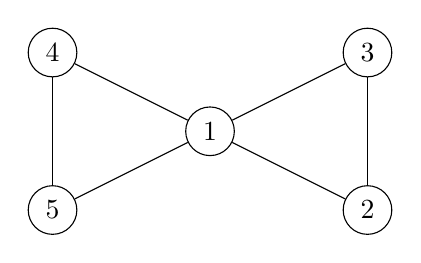
\begin{tikzpicture}
\node[circle,draw] (1) at (0,0){1};
\node[circle,draw] (2) at (2,-1){2};
\node[circle,draw] (3) at (2,1){3};
\node[circle,draw] (4) at (-2,1){4};
\node[circle,draw] (5) at (-2,-1){5};
\foreach \from/\to in {1/2,1/3,1/4,1/5,2/3,4/5}
  \draw (\from) -- (\to);
\end{tikzpicture}
\]
With Euler(ian) circuit (1231451).

A graph with both circuit is the simple $K_3$

\[
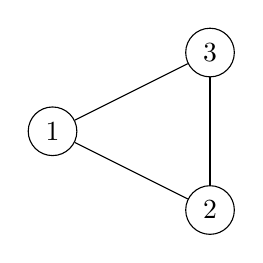
\begin{tikzpicture}
\node[circle,draw] (1) at (0,0){1};
\node[circle,draw] (2) at (2,-1){2};
\node[circle,draw] (3) at (2,1){3};
\foreach \from/\to in {1/2,1/3,2/3}
  \draw (\from) -- (\to);
\end{tikzpicture}
\]

With both the Euler(ian) and Hamilton(ian) circuits being (1231)


\newpage

Problem 6. Consider the following graph
\[
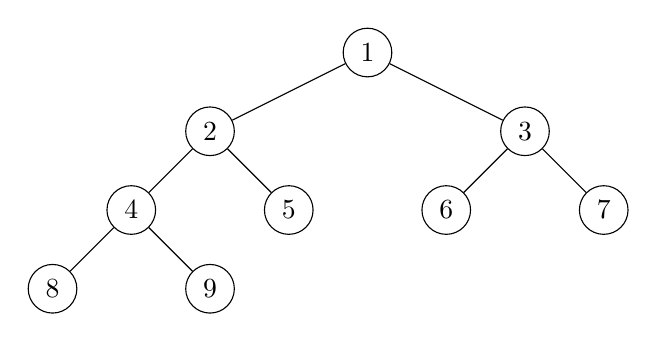
\begin{tikzpicture}
\node[circle,draw] (1) at (4,3){1};
\node[circle,draw] (2) at (2,2){2};
\node[circle,draw] (3) at (6,2){3};
\node[circle,draw] (4) at (1,1){4};
\node[circle,draw] (5) at (3,1){5};
\node[circle,draw] (6) at (5,1){6};
\node[circle,draw] (7) at (7,1){7};
\node[circle,draw] (8) at (0,0){8};
\node[circle,draw] (9) at (2,0){9};
\foreach \from/\to in {1/2,1/3,2/4,2/5,3/6,3/7,4/8,4/9}
  \draw (\from) -- (\to);
\end{tikzpicture}
\]

Write down the adjacency matrix for this graph.

\vspace{1in}
Since there are 9 vertices we will have a $9\times 9$ matrix.  Let's use the vertex labeling as in the demonstrated graph.

\[
\begin{bmatrix}
0 & 1 & 1 & 0 & 0 & 0 & 0 & 0 & 0\\
1 & 0 & 0 & 1 & 1 & 0 & 0 & 0 & 0\\
1 & 0 & 0 & 0 & 0 & 1 & 1 & 0 & 0\\
0 & 1 & 0 & 0 & 0 & 0 & 0 & 1 & 1\\
0 & 1 & 0 & 0 & 0 & 0 & 0 & 0 & 0\\
0 & 0 & 1 & 0 & 0 & 0 & 0 & 0 & 0\\
0 & 0 & 1 & 0 & 0 & 0 & 0 & 0 & 0\\
0 & 0 & 0 & 1 & 0 & 0 & 0 & 0 & 0\\
0 & 0 & 0 & 1 & 0 & 0 & 0 & 0 & 0\\
\end{bmatrix}
\]

\newpage

Problem 7. Consider the following matrix
\[
A = \begin{bmatrix}
1 & 0 & 1\\
0 & 1 & 0\\
1 & 0 & 2
\end{bmatrix}
\]

Compute $A^2$ and $A^3$.

\vspace{1in}

Solution:
\[
A^2 = \begin{bmatrix}
1 & 0 & 1\\
0 & 1 & 0\\
1 & 0 & 2
\end{bmatrix}
\begin{bmatrix}
1 & 0 & 1\\
0 & 1 & 0\\
1 & 0 & 2
\end{bmatrix} = \begin{bmatrix}
2 & 0 & 3\\
0 & 1 & 0\\
3 & 0 & 5
\end{bmatrix}
\]

and

\[
A^3 = A A^2 = \begin{bmatrix}
1 & 0 & 1\\
0 & 1 & 0\\
1 & 0 & 2
\end{bmatrix}  \begin{bmatrix}
2 & 0 & 3\\
0 & 1 & 0\\
3 & 0 & 5
\end{bmatrix} = 
\begin{bmatrix}
5 & 0 & 8\\
0 & 1 & 0\\
8 & 0 & 13
\end{bmatrix}
\]

Generally speaking (you need not know how to compute this)

\[
A^n = \begin{bmatrix}
F_{2n-1} & 0 & F_{2n}\\
0 & 1 & 0 \\
F_{2n} & 0 & F_{2n+1}
\end{bmatrix}
\]
where $F_j$ is the $j^{th}$ Fibonacci number $(F_0=0,F_1=1,F_2=1,F_3=2,F_4=3,F_5=5,\dots)$
\newpage

Bonus: Consider the complete bipartite graph $K_{20,20}$.  How many Euler(ian) circuits does this graph have?  How many Hamilton(ian) circuits?

\vspace{1in}

Solution: For the Hamiltonian $(20)!\times 20$.  
For the Euler(ian): extremely many.

\end{document}